
We discuss performance of the \ac{JSFRA} algorithm for different values of \me{\ell_q} over multiple time slots. It is compared with the existing \ac{Q-WSRME} scheme by varying the average arrival rate \me{A_k} of all users. Fig. \ref{fig-review} demonstrates the performance of the centralized algorithms for different \me{\ell_q} values. The horizontal axis indicates the average number of arrivals \me{A_k} in bits per user and it is constant for all users in the system. The vertical axis corresponds to the average of number of backlogged packets left in the system after each time slot. Even though \me{A_k}'s are constant for all users, the instantaneous arrivals are random and is based on Poisson arrival process. We considered a \me{4 \times 1} \ac{MIMO} system with \me{N = 4} sub-channels and \me{N_B = 2} \acp{BS}. The path loss is modeled as a uniform random variable \me{[0,-3]} dB with the maximum \ac{SINR} seen by any user is \me{6} dB. The average is performed over \me{100} slots.
\begin{figure}
\centering
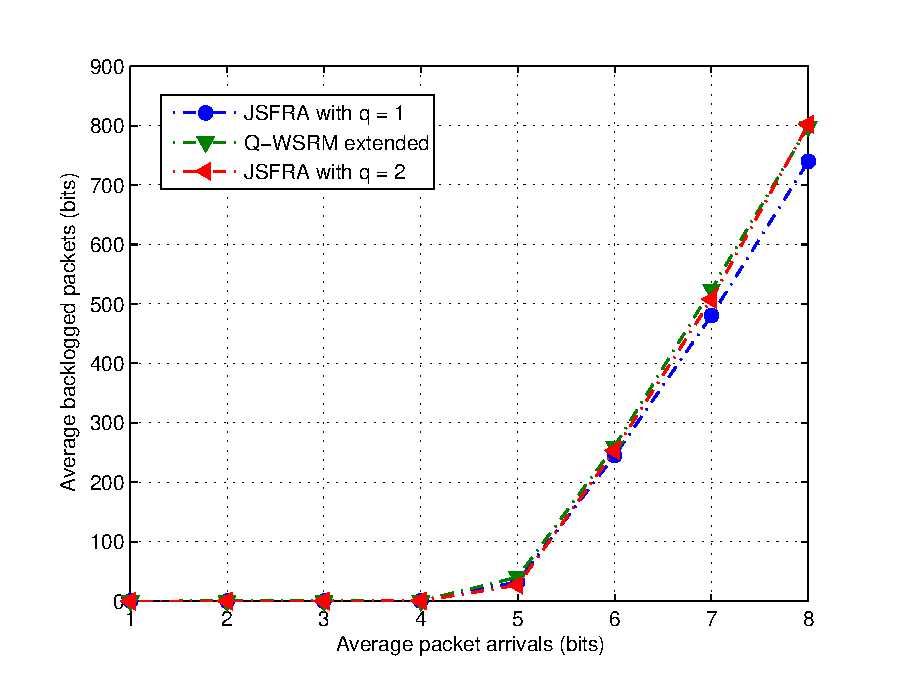
\includegraphics[width=\columnwidth]{Review/reviewer.eps}
\label{fig-review}
\caption{Average backlogged packets for different arrival rates with a system \me{\lbrace N,N_B,K,N_R \rbrace = \lbrace 4,2,12,1 \rbrace}}
\end{figure}

The performance of the \ac{JSFRA} scheme using \me{\ell_2} and \ac{Q-WSRME} approach are similar in the average number of residual packets after each transmission slot. Note that the additional rate constraints in the \ac{Q-WSRME} scheme is the reason for the equivalence. Both \ac{Q-WSRM} and \ac{Q-WSRME} performs similar to \me{\ell_2} \ac{JSFRA} scheme when the arrival rates are significantly greater than the actual transmissions. It can be seen from Fig. \ref{fig-review} that the average number of backlogged packets are noticeably less for the \me{\ell_1} \ac{JSFRA} formulation due to the greedy resource allocation by serving users with better channel conditions. Fig \ref{fig-review} shows that the \me{\ell_{\infty}} \ac{JSFRA} scheme performs worst in terms of the average number of backlogged packets due to the fairness constraints.